\chapter{Internetska aplikacija}

Internetska aplikacija se sastoji od korisni\v{c}kog su\v{c}elja za internetske korisnike i (API) za mobilne korisnike. Zajedni\v{c}ko objema aplikacijama je kori\v{s}tenje iste baze podataka koja slu\v{z}i kao centralni repozitorij podataka. U nastavku ovog poglavlja je prvo obja\v{s}njena struktura baze, a zatim implementacija internetske aplikacije i API su\v{c}elja.

\section{Baza podataka}

Baza podataka se sastoji od \v{s}est tablica te je modelirana po tre\'{c}oj normalnoj formi. To zna\v{c}i da su tablice kreirane i pomo\'{c}u relacijskih veza strukturirane s ciljem minimiziranja redundancije podataka. Relacijske veze uklju\v{c}uju definiranje primarnog klju\v{c}a svake tablice (atribut tablice koji ima jedinstvenu vrijednost za svaki zapis) te kreiranje stranih klju\v{c}eva (veza izme\dj u primarnog klju\v{c}a jedne tablice i atributa druge tablice). Struktura baze i veze izme\dj u tablica su prikazani na slici ~\ref{fig:bazaPodataka}.


\begin{figure}[!htbp]
	\begin{center}
 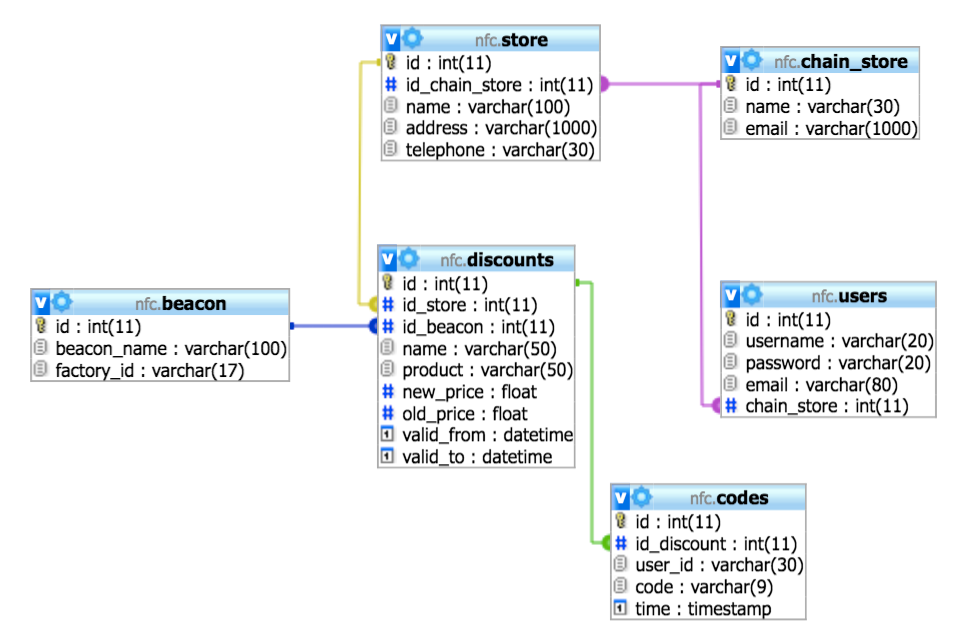
\includegraphics[height=10cm,keepaspectratio=true]{web_baza}
 \caption{Struktura baze podataka}
 \label{fig:bazaPodataka}
	\end{center}
\end{figure}

Baza podataka se sastoji od slijede\'{c}ih tablica:
\begin{itemize}
	\item Lanac trgovina
	\begin{itemize}
		\item Sadr\v{z}i naziv i e-mail adresu lanca trgovina
	\end{itemize}
	\item Poslovnica
	\begin{itemize}
		\item Sadr\v{z}i osnovne informacije o poslovnici i referencu na lanac trgovina
	\end{itemize}
	\item Popust
	\begin{itemize}
		\item Sadr\v{z}i osnovne informacije o popustu i referencu na poslovnicu i ogla\v{s}iva\v{c}
	\end{itemize}
	\item Ogla\v{s}iva\v{c}
	\begin{itemize}
		\item Sadr\v{z}i naziv i strojnu adresu ogla\v{s}iva\v{c}a
	\end{itemize}
	\item Kod za popust
	\begin{itemize}
		\item Sadr\v{z}i kod, vrijeme aktivacije i identifikator korisnika te referencu na popust
	\end{itemize}
	\item Korisnik
	\begin{itemize}
		\item Korisnik internetske aplikacije, vezan je za lanac trgovina
	\end{itemize}
\end{itemize}



\section{Internetska aplikacija}

\subsection{Su\v{c}elje za pristup}

Prvo \v{s}to korisnik vidi kada preko pretra\v{z}iva\v{c}a ode na lokaciju internetske aplikacije je forma za unos kredencija, prikazana na slici ~\ref{fig:webLogin}. Korisnik je du\v{z}an unjeti svoje korisni\v{c}ko ime i lozinku, kako bi pristupio po\v{c}etnom su\v{c}elju.

\begin{figure}[!htbp]
	\begin{center}
 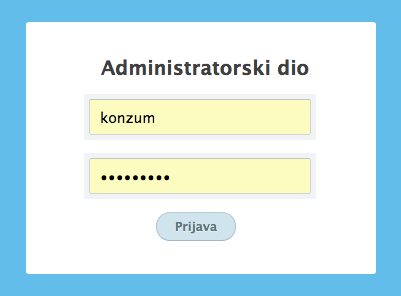
\includegraphics[height=5cm,keepaspectratio=true]{web_login}
 \caption{Forma za unos kredencija}
 \label{fig:webLogin}
	\end{center}
\end{figure}


\subsection{Po\v{c}etno su\v{c}elje}

Nakon uspje\v{s}nog pristupanja aplikaciji, korisniku je prikazano po\v{c}etno su\v{c}elje na slici ~\ref{fig:web_glavni}. Su\v{c}elje se sastoji od izbornika, centralnog dijela i tipke za odjavu iz sustava. U izborniku se nalaze glavne korisni\v{c}ke opcije koje uklju\v{c}uju popis poslovnica, su\v{c}elje za kreiranje popusta i su\v{c}elje za kreiranje nove poslovnice.


\begin{figure}[!htbp]
	\begin{center}
 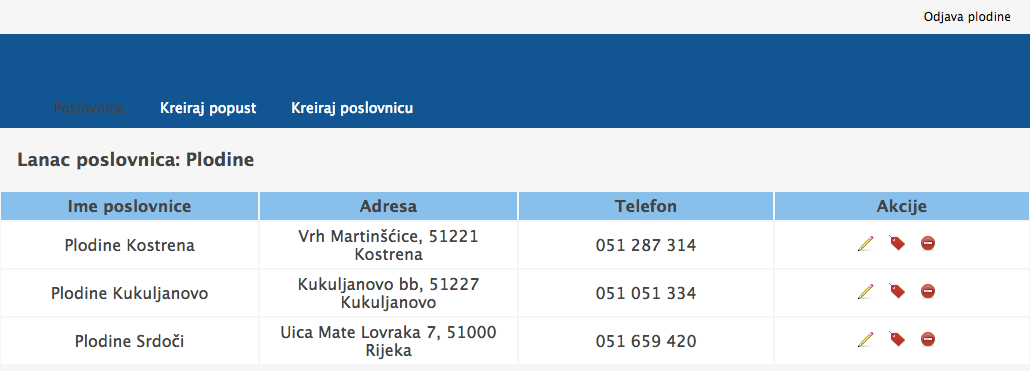
\includegraphics[height=5cm,keepaspectratio=true]{web_glavni}
 \caption{Popis poslovnica trgova\v{c}kog lanca}
 \label{fig:web_glavni}
	\end{center}
\end{figure}

Kada se korisnik prijavi u sustav u centralnom dijelu su\v{c}elja mu se prika\v{z}e popis poslovnica trgova\v{c}kog lanca za kojeg je vezan. Popis je prikazan u formatu tablice te osim osnovnih informacija o poslovnicama uklju\v{c}uje i akcije vezane za poslovnicu. Dostupne akcije su ure\dj enje poslovnice, pregledavanje popusta poslovnice i brisanje poslovnice.


\subsection{Poslovnica}

U aplikaciji je implementirano dodavanje, ure\dj ivanje i brisanje poslovnice, a oggovaraju\'{c}a su\v{c}elja si prikazana na slici ~\ref{fig:web_poslovnicaa}.

\begin{figure}[!htbp]
	\begin{center}
 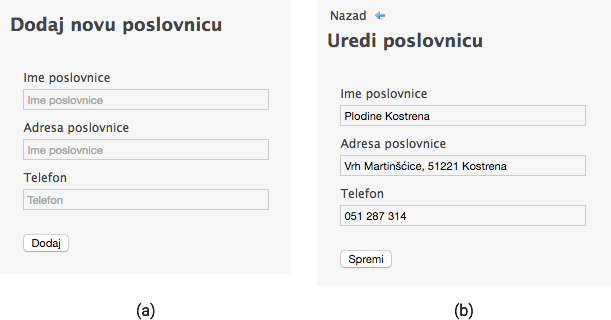
\includegraphics[height=7cm,keepaspectratio=true]{web_poslovnicaa}
 \caption{Dodavanje i ure\dj ivanje poslovnice}
 \label{fig:web_poslovnicaa}
	\end{center}
\end{figure}

Korisnik sa popisa poslovnica mo\v{z}e odabrati i pregled popusta poslovnice, te mu se tada u centralnom dijelu su\v{c}elja prikazuju svi popusti poslovnice, prikazani na slici ~\ref{fig:web_popusti}.

\begin{figure}[!htbp]
	\begin{center}
 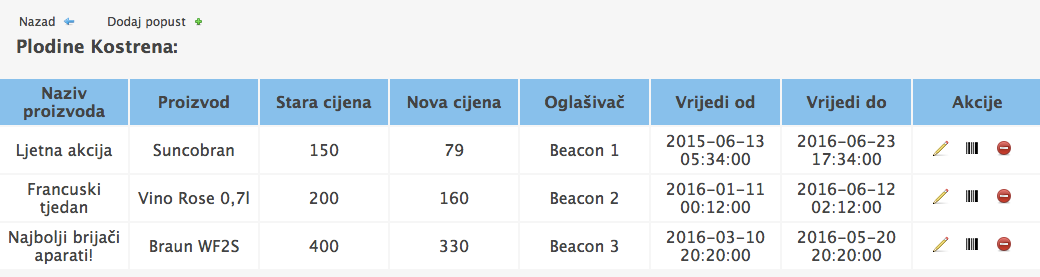
\includegraphics[height=3.9cm,keepaspectratio=true]{web_popusti}
 \caption{Popusti poslovnice}
 \label{fig:web_popusti}
	\end{center}
\end{figure}

Popusti su strukturirani u tablicu iz koje korisnik mo\v{z}e pro\v{c}itati podatke o popustu, kao i napraviti akcije koje uklju\v{c}uju ure\dj ivanje i brisanje popusta te pregled aktivacijskih kodova poslovnice.


\subsection{Popust}

Korisniku je omogu\'{c}eno kreiranje, ure\dj ivanje i brisanje popusta. Na slici ~\ref{fig:web_dodaj_popust} su prikazane forme za kreiranje i ure\dj ivanje popusta.

\begin{figure}[!htbp]
	\begin{center}
 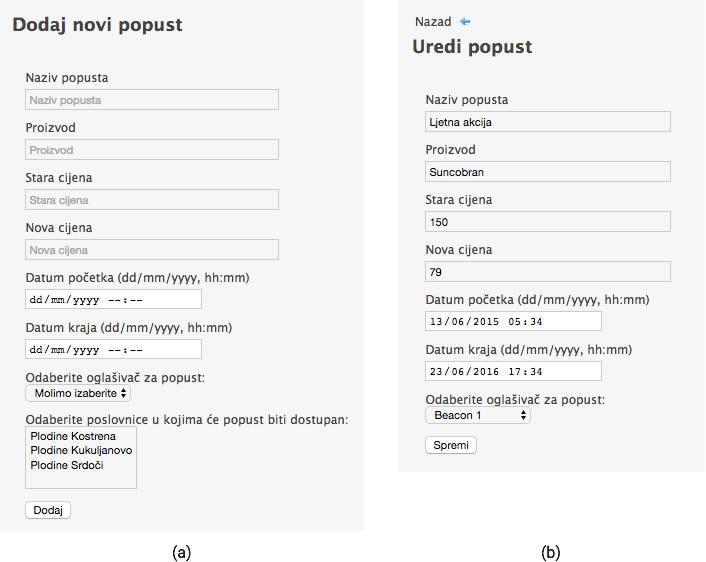
\includegraphics[height=10cm,keepaspectratio=true]{web_dodaj_popust}
 \caption{Popusti poslovnice}
 \label{fig:web_dodaj_popust}
	\end{center}
\end{figure}
Kod kreiranja popusta je potrebno unjeti osnovne informacije o popustu koje uklju\v{c}uju i ogla\v{s}iva\v{c} za kojeg je popust vezan, kao i poslovnice u kojim se popust mo\v{z}e ostvariti. Kod ure\dj ivanja popusta koji je ve\'{c} vezan za poslovnicu korisnik mo\v{z}e, uz osnovne informacije, promjeniti samo ogla\v{s}iva\v{c} za kojeg je popust vezan.


\subsection{Pregled kodova popusta}
Za svaku popust u poslovnici je mogu\'{c}eno i pregledavanje kodova koji su izdani za popuste. Primjer aktiviranih kodova je prikazan na slici ~\ref{fig:web_kodovi}.

\begin{figure}[!htbp]
	\begin{center}
 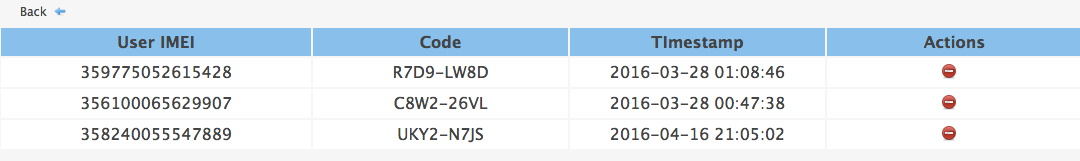
\includegraphics[height=2.2cm,keepaspectratio=true]{web_kodovi}
 \caption{Aktivirani kodovi popusta}
 \label{fig:web_kodovi}
	\end{center}
\end{figure}

Na su\v{c}elju su prikazane informacije o popustu koje uklju\v{c}uju identifikator korisnika (IMEI broj njegovog pametnog telefona), aktivacijski kod, vrijeme aktiviranja koda i opcija brisanja aktivacije.

\subsection{API su\v{c}elje}

API su\v{c}elje ozna\v{c}ava skup pravila komunikacije kojeg koriste dva ra\v{c}unalna sustava kako bi razmijenili informacije. U sklopu ovog projekta je su\v{c}elje moralo biti implementirano kako bi mobilna aplikacija mogla komunicirati sa bazom podataka koju koristi internetska aplikacija. Komunikacija se vr\v{s}i tako da mobilna aplikacija radi API zahtjev sa ispravom metodom (GET ili POST) na ispravnu internetsku lokaciju. Ovisno o tipu komunikacije, zahtjev mora sadr\v{z}avati odre\dj ene podatke kako bi su\v{c}elje znalo napraviti ispravan zahtjev prema bazi (primjer je aktivacija popusta pri \v{c}emu je mobilna aplikacija u zahtjevu du\v{z}na poslati ure\dj ajev IMEI). Kada su podaci izvu\v{c}eni iz baze podataka, potrebno ih je serijalizirati u format koji je podoban za slanje i kojeg primatelj zna interpretirati. Za potrebe ove aplikacije je kori\v{s}ten JSON format \cite{json} (JavaScript Object Notation), koji specificira podatke kao kolekciju parova ime-vrijednost. Vrijednost mo\v{z}e biti primitiv, objekt i lista primitiva/objekta. Na slici ~\ref{fig:web_json} je prikazana konfiguracija poslovnice koja se \v{s}alje preko API-a, u JSON formatu.


\begin{figure}[!htbp]
	\begin{center}
 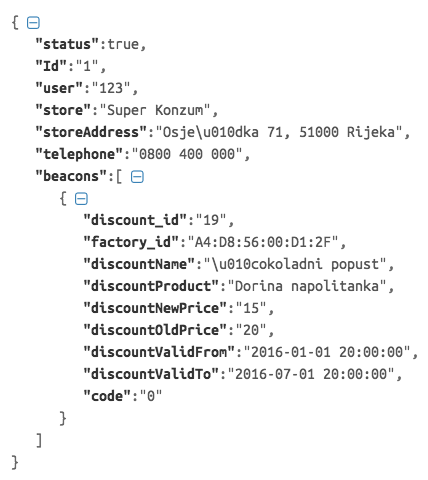
\includegraphics[height=9cm,keepaspectratio=true]{web_json}
 \caption{Aktivirani kodovi popusta}
 \label{fig:web_json}
	\end{center}
\end{figure}







